
%(BEGIN_QUESTION)
% Copyright 2014, Tony R. Kuphaldt, released under the Creative Commons Attribution License (v 1.0)
% This means you may do almost anything with this work of mine, so long as you give me proper credit

Calculate the voltage output by this 4:1 step-down transformer ($V_X$, with reference to ground) with its primary winding connected to two lines of a three-phase bus, given the phase voltages of the bus shown below:

$$\includegraphics[width=15.5cm]{i03113x01.eps}$$

$V_A$ = 600 V $\angle$ 0$^{o}$ \hskip 20pt $V_B$ = 600 V $\angle$ $-120^{o}$ \hskip 20pt $V_C$ = 600 V $\angle$ $120^{o}$

\vskip 10pt

Your answer needs to specify both the magnitude of $V_X$ as well as its phase angle:

\vskip 10pt

$V_X$ = \underbar{\hskip 80pt} 

\underbar{file i03113}
%(END_QUESTION)





%(BEGIN_ANSWER)

$V_X$ = 259.8 V $\angle$ $-90^o$ \hskip 10pt or \hskip 10pt 259.8 V $\angle$ $270^o$
 
%(END_ANSWER)





%(BEGIN_NOTES)

{\bf This question is intended for exams only and not worksheets!}.

%(END_NOTES)


